Como visto no capítulo anterior \ref{chapter:bibliotecas_do_ruby}, a maior parte das bibliotecas do
\emph{Ruby} são distribuídas na forma de \emph{gems}, e também vimos na seção
\ref{subsection:programa_gem} que a ferramenta \emph{gem} é um sistema de distribuição
% similar ao  \emph{\href{https://packages.qa.debian.org/a/apt.html}{apt-get}},
que facilita o compartilhamento e a instalação de \emph{gemas}.

Este capítulo tem o objetivo de mostrar um passo-a-passo para criar uma gema.
Apresentaremos primeiramente uma modelo de criação de gemas na seção \ref{section:modelo_de_criação}.
Depois na seção \ref{section:processo_de_criação}, vamos mostrar na prática como realizar os passos indicados
na seção \ref{section:modelo_de_criação}. E por fim na seção \ref{section:exemplo_de_criação}, apresentaremos um
exemplo, criando uma gema que faz a tradução de algumas palavras do português para o inglês. Para obter informações
sobre as ferramentas utilizadas e de como preparar o ambiente de desenvolvimento, consulte os apêndices
\ref{chapter:ferramentas_utilizadas} e \ref{chapter:preparação_do_ambiente}, respectivamente.


\section{Modelo de Criação}
\label{section:modelo_de_criação}


O primeiro passo para se criar uma gema, é construir uma solução de um certo problema que será utilizado
com frequência. Por exemplo, a função que calcula a raiz quadrada.

Após encontrar uma ideia para a criação de uma gema, deve-se elaborar um projeto, fazendo o levantamento
de requisitos, o \emph{design}, a implementação, os testes e a entrega. Por simplificação, somente
apresentaremos a parte de implementação do modelo de criação.

Quando o projeto chegar no momento da implementação, devemos criar um diretório com o nome do projeto.
Dentro deste diretório, vamos inserir todos os códigos relacionados a biblioteca, como por exemplo, a
descrição, a versão, os códigos de funcionalidades, e os códigos de testes.

Após a criação do diretório do projeto, devemos criar um arquivo com a descrição da biblioteca. Esta
descrição deve conter informações básicas, como por exemplo, o nome, a descrição, os autores, os
contatos, e as dependências da biblioteca.

Com o arquivo da descrição criado, devemos determinar uma versão para a biblioteca, pois desta forma
além de construirmos um histórico, podemos marcar e resgatar versões estáveis do projeto.

Com a descrição e a versão da biblioteca determinados, iniciamos o processo de criação de código.
Esse processo possui dois tipos de desenvolvimento. O desenvolvimento de códigos de
funcionalidades que consiste na implementação das funcionalidades da gema. E o desenvolvimento
de códigos de testes que serve determinar a corretude das funcionalidades.

Por fim, após a implementação dos dois tipos de códigos, devemos realizar a execução dos testes
para confirmar que as funcionalidades foram implementadas de forma correta.

Para agilizar o processo de implementação, a comunidade do \emph{Ruby}, desenvolveu ferramentas para
facilitar a criação de aplicações e bibliotecas. Estas ferramentas são acionados por meio de
linhas de comando para criar automaticamente esqueletos de aplicações ou bibliotecas. Estes esqueletos
possuem arquivos com informações básicas que geralmente são utilizadas no desenvolvimento. Veremos
mais detalhes sobre esse assunto na próxima seção.


\section{Processo de Criação}
\label{section:processo_de_criação}


Esta seção, tem o objetivo de mostrar detalhadamente a estrutura básica de uma gema, e também apresentar
detalhadamente os passos do modelo de criação, vistos na seção \ref{section:modelo_de_criação}.

Deste modo, antes de iniciarmos o processo de criação, na seção \ref{subsection:estrutura}, vamos analisar
detalhadamente todos os elementos da estrutura básica de uma gema, e depois com o este conhecimento
adquirido, vamos mostrar na seção \ref{subsection:modelo_de_criação_detalhado}, o modelo de criação detalhado.


\subsection{Estrutura}
\label{subsection:estrutura}


Uma gema do \emph{Ruby}, obrigatoriamente deve possui um nome, um número de versão e uma plataforma.
Internamente ela deve possuir códigos de funcionalidade, uma documentação, e um \emph{\textbf{gemspec}},
explicado abaixo.

A sua estrutura geralmente é organizada em 3 arquivos bases: o \emph{\textbf{gemspec}}, o
\emph{\textbf{Rakefile}} e o \emph{\textbf{README}}, e em 3 diretórios principais: \emph{\textbf{bin}},
\emph{\textbf{lib}}, e \emph{\textbf{test}} ou \emph{\textbf{spec}}. Na listagem abaixo veremos para que
serve cada um destes arquivos e diretórios.

\begin{itemize}

 \item O \emph{\textbf{gemspec}} é um arquivo com extensão ‘‘\emph{.gemspec}'' que possui as informações básicas
 de uma gema, como por exemplo o seu nome, sua descrição, seu autor, seu endereço, e suas dependências.

 \item O \emph{\textbf{bin}} é um diretório que possui arquivos de bibliotecas, usados pelo \emph{Ruby}.
 Estas bibliotecas são carregadas quando a gema for instalada.

 \item O \emph{\textbf{lib}} é um diretório que possui todos os códigos \emph{Ruby} referentes ao
 funcionamento da gema.

 \item O \emph{\textbf{Rakefile}} é um arquivo que possui código \emph{Ruby} que faz a otimização de algumas
 funcionalidades por meio da execução do programa \emph{\href{https://github.com/jimweirich/rake}{rake}}
 \footnote{rake: \url{https://github.com/jimweirich/rake}}. Um exemplo, é a execução de todos os arquivos
 de testes do diretório \emph{test} ou \emph{spec}.

 \item O \emph{\textbf{test}} ou \emph{\textbf{spec}} é um diretório que possui todos os códigos \emph{Ruby}
 de testes. Eles podem ser executados manualmente ou por meio do \emph{Rakefile}.

 \item O \emph{\textbf{README}} é um arquivo que usualmente possui a documentação da gema. Esta
 documentação, usualmente é retirada de comentários que estão dentro do código, e gerados automaticamente
 quando a gema é instalada. A maioria das gemas possuem a documentação
 \emph{\href{http://rdoc.sourceforge.net/doc/}{RDoc}} \footnote{RDoc: \url{http://rdoc.sourceforge.net/doc/}},
 e as outras, em minoria, possuem a documentação \emph{\href{http://yardoc.org/}{YARD}}
 \footnote{YARD: \url{http://yardoc.org/}} [\citeonline{guide_what_is_a_gem_rubygems}].

\end{itemize}


\subsection{Modelo de Criação Detalhado}
\label{subsection:modelo_de_criação_detalhado}


Esta seção tem o objetivo de mostrar detalhadamente o processo de criação de uma gema.
Apresentaremos na seção \ref{subsubsection:criando_a_estrutura}, uma forma de criação automatica da
estrutura básica de uma gema. Depois na seção \ref{subsubsection:inserindo_descrição},
apresentaremos como inserir os detalhes sobre a gema. Em seguida, na seção
\ref{subsubsection:desenvolver_funcionalidades_ou_testes}, apresentaremos que existe a possibilidade
de escolher entre, implementar os códigos de funcionalidades e depois os códigos de testes, ou
implementar os códigos de testes e depois implementar os códigos de funcionalidades. Depois na seção
\ref{subsubsection:desenvolver_funcionalidades}, apresentaremos como inserir os códigos de testes. Em
seguida, apresentaremos na seção \ref{subsubsection:desenvolver_testes}, como inserir os
códigos de testes.


\subsubsection{Criando a Estrutura}
\label{subsubsection:criando_a_estrutura}


O primeiro passo é fazer a criação da estrutura da gema e isso pode ser feito de forma manual ou automatica.
A forma manual implica em criar todos os diretórios e arquivos manualmente. A forma automatica implica na
execução de um simples comando.

Podemos perceber que a forma manual não é muito aconselhável, pois perderiamos muito tempo criando
os arquivos e também poderiamos cometer erros no momento da criação, como por exemplo, escrever errado
o nome de algum arquivo ou diretório. Por estes motivos, utilizaremos a forma automatica
que além de criar a estrutura, prepara um código base dentro dos arquivos.

A execução do comando \textbf{‘‘ \emph{bundle gem ‘ nome da gema'} ''} no terminal, faz a criação da
estrutura básica de forma automatica. Neste caso, ‘‘\emph{nome da gema}'' pode ser o nome do projeto
da biblioteca.

Mais detalhes sobre a criação da estrutura serão abordados no exemplo apresentado na seção
\ref{subsection:criando_a_estrutura_automaticamente}.


\subsubsection{Inserindo Descrição}
\label{subsubsection:inserindo_descrição}


Após criar a estrutura básica da gema, devemos fazer a edição do arquivo \emph{\textbf{gemspec}}
para informar os dados básicos da gema, e isso pode ser feito editando o arquivo ‘‘ \emph{'nome da gema'.gemspec }''.

Detalhes como, autores e e-mails servem para informar quem criou e como se comunicar com os donos da gema,
nome e descrição servem para informar o objetivo da gema, e dependências servem para informar quais as bibliotecas
são necessárias para o uso da gema.

Mais detalhes sobre o arquivo ‘‘ \emph{'nome da gema'.gemspec }'', serão abordados no exemplo na seção
\ref{subsection:editando_gemspec}.


\subsubsection{Desenvolver Funcionalidades ou Testes}
\label{subsubsection:desenvolver_funcionalidades_ou_testes}


Nesse momento, depois de detalharmos a gema no gemspec, podemos tomar 2 caminhos. Neste caso, o caminho a ser
tomado é depende da metodologia de projeto adotada no inicio do desenvolvimento, ou seja, é nesse
momento que podemos desenvolver os códigos das funcionalidades ou implementar os códigos de testes.

Na metodologia tradicional se faz a implementação dos códigos de funcionalidades e depois se
desenvolve os códigos para testar as funcionalidades. Por outro lado, na metodologia voltada para
testes, se implementa os códigos de testes para depois se desenvolver os códigos de funcionalidades.

Seguindo a metodologia tradicional, primeiramente iremos fazer o código das funcionalidades da gema.
Depois ao terminar de criar as funcionalidades, iremos elaborar os arquivos de testes. Mas nada o impede
de desenvolver os códigos de testes que serão apresentado na seção \ref{subsubsection:desenvolver_testes},
antes de desenvolver os códigos de funcionalidade, mostrados na seção
\ref{subsubsection:desenvolver_funcionalidades}.


\subsubsection{Desenvolver Funcionalidades}
\label{subsubsection:desenvolver_funcionalidades}


Caso os códigos de funcionalidades sejam desenvolvidos por meio de código \emph{Ruby}, devemos fazer a
edição e a criação de arquivos no diretório \emph{\textbf{lib}}. Este diretório obrigatoriamente deve
possuir um arquivo ‘‘ \emph{'nome da gema'.rb }'' e um diretório, também com o nome da gema, com um arquivo
de versão com o nome ‘‘\emph{version}''.

Basicamente a descrição da versão de uma gema é uma \emph{string} com números e pontos. Também é permitido
colocar ao final a palavra chave ‘‘\emph{pre}'', caso seja um pré-lançamento de alguma versão.
Por exemplo, ‘‘\emph{1.0.0.pre}'' é um pré-lançamento da versão ‘‘\emph{1.0.0}''.

O \emph{Rubygems} recomenda seguir as seguintes políticas mencionadas logo abaixo que foram consultadas
em \emph{\href{http://guides.rubygems.org/patterns/\#semantic-versioning}{semantic-versioning}}
\footnote{semantic-version: \url{http://guides.rubygems.org/patterns/\#semantic-versioning}} e em
\emph{\href{http://guides.rubygems.org/specification-reference/\#version}{specification-reference-version}}
\footnote{specification-reference-version: \url{http://guides.rubygems.org/specification-reference/\#version}}.

\begin{itemize}
 \item \emph{PATH}: “0.0.X” para pequenas alterações, como por exemplo correção de pequenos \emph{bugs}.
 \item \emph{MINOR}: “0.X.0” para médias alterações, como por exemplo alteração/adição de funcionalidades.
 \item \emph{MAJOR}: “X.0.0” para grandes alterações, como por exemplo remoção de alguma funcionalidade.
\end{itemize}


No arquivo ‘‘\emph{lib/'nome da gema'.rb}'' temos a possibilidade de escrever todas as
funcionalidades desejadas. No entanto é recomendado fazer a modularização por meio do comando
 ‘‘\emph{require}'' que é utilizado para fazer a chamada de código de outros
arquivos.

Por exemplo, suponha que desenvolvemos uma gema e depois de um certo tempo precisamos fazer a manutenção do
seu código. Neste caso, se não modularizamos a gema, a correção de \emph{bugs} ou mesmo a adição de
novas funcionalidades, torna-se uma tarefa muito complexa, pois não existe nenhuma organização
estrutural na gema preparada para facilitar esse tipo de operação.

Mais detalhes sobre o arquivo ‘‘\emph{lib/'nome da gema'.rb} '' e os outros códigos de funcionalidades do
diretório ‘‘ \emph{lib/'nome da gema'} '', serão abordados no exemplo na seção
\ref{subsection:codigo_de_funcionalidade_no_diretorio_lib}.


\subsubsection{Desenvolver Testes}
\label{subsubsection:desenvolver_testes}


Para se fazer os testes, deve-se criar os arquivos de testes dentro do diretório ‘‘\textbf{\emph{test}}'' ou se
preferir ‘‘\textbf{\emph{spec}}''. Não existe um padrão especificado, mais recomenda-se criar um arquivo de
teste com o nome ‘‘\emph{test/test\_‘definição do teste'.rb}''. Neste caso, ‘‘\emph{definição do teste}''
descreve o nome do teste a ser realizado, como por exemplo, para o arquivo
‘‘\emph{test/test\_raiz\_quadrada.rb}'', testa a função que calcula a raiz quadrada.

Após a criação dos arquivos de testes, é recomendado fazer a criação do arquivo ‘‘\textbf{\emph{Rakefile}}'' para
automatizar os testes. Deste modo, quando for necessário testar a gema, não será necessário chamar teste
por teste, pois todas as chamadas de teste estarão determinadas no arquivo ‘‘\textbf{\emph{Rakefile}}''.

Vale ressaltar que no momento do desenvolvimento dos códigos de testes, é aconselhável implementar testes
para cada função da gema, verificado se para todas as entradas possíveis, se recebe o resultado
esperado.

Mais detalhes sobre os arquivos de testes e o arquivo ‘‘\textbf{\emph{Rakefile}}'', serão abordados no exemplo
na seção \ref{subsection:codigo_de_teste_no_diretorio_test_ou_spec}.


\section{Exemplo de Criação}
\label{section:exemplo_de_criação}


Esta seção tem o objetivo de mostrar um exemplo de criação de uma gema utilizando o modelo de criação.
Para o exemplo, vamos fazer a criação da gema
\emph{\href{https://github.com/toshikomura/gemtranslatetoenglish/tree/without_path}{gemtranslatetoenglish}}
\footnote{gemtranslatetoenglish : \url{https://github.com/toshikomura/gemtranslatetoenglish/tree/without_path}},
que tem como objetivo, fazer a tradução de um texto em português para um texto em inglês.

Futuramente pretendemos aumentar o vocabulário da gema de exemplo, mas até o momento de término deste
trabalho, ela possuía somente a tradução de duas palavras, ‘‘\emph{OLÁ}'' para ‘‘\emph{HELLO}'' e
‘‘\emph{MUNDO}'' para ‘‘\emph{WORLD}''. Apesar de possuir pouco vocabulário, a gema ‘‘\emph{gemtranslatetoenglish}''
possui características suficientes para a apresentação do tutorial deste trabalho.

Nesta seção, vamos apresentar na seção \ref{subsection:criando_a_estrutura_automaticamente}, a criação da
estrutura básica. Depois na seção \ref{subsection:editando_gemspec}, vamos mostrar como detalhar a gema no
arquivo ‘‘\emph{gemspec}''. Em seguida, na seção \ref{subsection:codigo_de_funcionalidade_no_diretorio_lib},
vamos mostrar a criação dos códigos de funcionalidades. Depois vamos apresentar na seção
\ref{subsection:codigo_de_teste_no_diretorio_test_ou_spec}, a criação dos códigos de testes. E por fim na
seção \ref{subsection:exemplo_de_uso_da_biblioteca_criada}, apresentaremos um exemplo do uso da gema
‘‘\emph{gemtranslatetoenglish}'' em um projeto \emph{Ruby On Rails}.


\subsection{Criando a Estrutura Automaticamente}
\label{subsection:criando_a_estrutura_automaticamente}


No caso da nossa gema de exemplo, foi feita a execução do comando \textbf{‘‘\emph{bundle gem gemtranslatetoenglish}''}
para fazer a criação da estrutura básica de forma automatica. Ao se fazer a execução deste comando de criação, obtemos
a seguinte estrutura de gema mostrada no código \ref{lst:execucao_que_cria_gema_gemtranslatetoenglish}.

%\lstinputlisting[ style=customBash, caption={Cria Gema gemtranslatetoenglish}, label={lst:cria_gema_gemtranslatetoenglish}]
%{codigos/cria_gema_gemtranslatetoenglish.sh}

% na imagem ‘‘Figura \ref{fig:execucao_que_cria_gema_gemtranslatetoenglish} - Execução que cria gema gemtranslatetoenglish''.

\lstinputlisting[ style=customBash, caption={Execução que cria gema gemtranslatetoenglish}, label={lst:execucao_que_cria_gema_gemtranslatetoenglish}]
{codigos/execucao_que_cria_gema_gemtranslatetoenglish.sh}

Podemos perceber que no código \ref{lst:execucao_que_cria_gema_gemtranslatetoenglish}, foi feita a criação do
diretório ‘‘\emph{gemtranslatetoenglish}'' com os arquivos ‘‘\emph{Gemfile}'', ‘‘\emph{Rakefile}'',
‘‘\emph{LICENCE.txt}'', ‘‘\emph{README.md}'', ‘‘\emph{.gitignore}'', ‘‘\emph{gemtranslatetoenglish.gemspec}'',
e o diretório ‘‘\emph{lib}''. E dentro do diretório ‘‘\emph{lib}'' foi criado o arquivo
‘‘\emph{gemtranslatetoenglish.rb}'', e o diretório ‘‘\emph{gemtranslatetoenglish}'' com o arquivo
‘‘\emph{version.rb}'' dentro dele.

\begin{comment}
\begin{figure}[ht]
  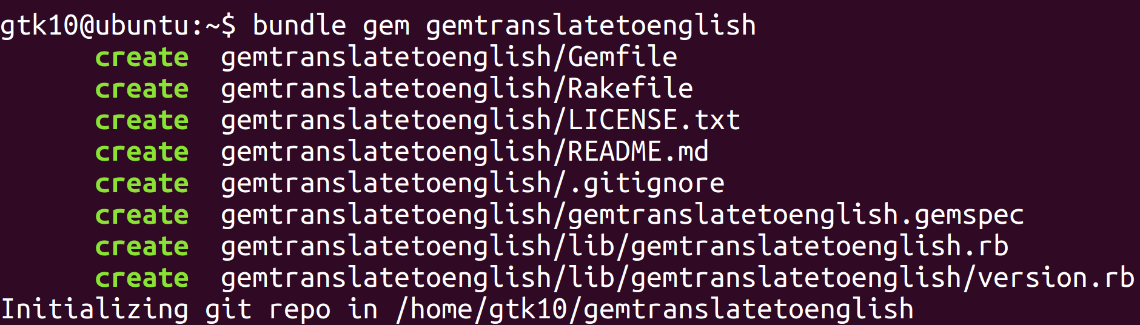
\includegraphics[scale=0.4]{images/execucao_que_cria_gema_gemtranslatetoenglish}
  \caption{Execução que cria gema gemtranslatetoenglish}
  \label{fig:execucao_que_cria_gema_gemtranslatetoenglish}
\end{figure}
\end{comment}


\subsection{Editando Gemspec}
\label{subsection:editando_gemspec}


No nosso exemplo, para detalharmos a gema, fizemos a edição do arquivo ‘‘gemtranslatetoenglish.gemspec'',
resultado no arquivo mostrado no código \ref{lst:gemspec_gemtranslatetoenglish}.
%na imagem ‘‘Figura \ref{fig:gemspec_gemtranslatetoenglish} - gemspec gemtranslatetoenglish''
Cada linha deste código será explicada com mais detalhes logo a seguir.

\lstinputlisting[ style=customBash, caption={gemspec gemtranslatetoenglish}, label={lst:gemspec_gemtranslatetoenglish}]
{codigos/gemtranslatetoenglish/gemtranslatetoenglish.gemspec}


\begin{itemize}

 \item ‘‘\emph{\# coding: utf-8}'' na linha ‘‘1'' indica que o texto do arquivo está no formato \emph{UTF-8}.

 \item ‘‘\emph{lib = File.expand\_path('..\/lib', \_\_FILE\_\_)}'' na linha ‘‘2'' indica onde se encontra o
 diretório \emph{\textbf{lib}} da gema.

 \item ‘‘\emph{\$LOAD\_PATH.unshift(lib) unless \$LOAD\_PATH.include?(lib)}'' na linha ‘‘3'' faz o
 carregamento dos arquivos que estão no diretório \emph{\textbf{lib}}, somente se o diretório já
 esta definido.

 \item ‘‘ \emph{require 'gemtranslatetoenglish/version'} '' na linha ‘‘4'' requisita a versão da gema.

 \item ‘‘\emph{Gem::Specification.new do |spec|} ... end'' da linha ‘‘6'' a ‘‘23'' define a especificação da
 gema como \emph{spec}, ou seja, ao invés de escrever ‘‘\emph{Gem::Specification}'' a todo momento que for
 definir uma especificação da gema se escreve somente ‘‘\emph{spec}''.

 \item ‘‘\emph{spec. }'' da linha ‘‘7'' a linha ‘‘14'' defini-se especificações básicas da gema, como nome,
 versão, autor, e-mail do autor, breve descrição, descrição completa, página e tipo de licença.

 \item ‘‘\emph{spec.files = `git ls-files -z`.split("$\backslash$x0")}'' na linha ‘‘16'' indica os arquivos
 que devem ser incluídos na gema. Esses arquivos são incluídos dinâmicamente através do comando
 ‘‘\emph{git ls-files -z}''. Este comando do \emph{git}, traz como resultado todos os arquivos que estão
 naquele repositório, colocando entre as \emph{PATH}s, o caracter ‘‘\emph{$\backslash$0}''
 (\emph{line termination on output}). Por consequência, com a adição do comando \emph{Ruby}
 ‘‘\emph{.split("$\backslash$x0")}'', é feita a divisão por ‘‘\emph{$\backslash$0}'', separando as
 \emph{PATH}s dos arquivos. Deste modo, os arquivos adicionados na gema, são todos que estão no repositório.

 Para se adicionar arquivos no repositório é necessário executar o comando ‘‘\emph{git add PATH}'',
 onde \emph{PATH} é o caminho do arquivo que se deseja adicionar no repositório.

 \item ‘‘\emph{spec.executables = ...}'' e ‘‘\emph{spec.tes\_files = ...}'' nas linhas ‘‘17'' e ‘‘18''
 indicam os arquivos executáveis e os arquivos de teste respectivamente. Também indica que os arquivos dentro
 destes diretórios, devem ter permissão de execução.

 \item ‘‘\emph{spec.require\_paths = ["lib"]}'' requisita o diretório da \emph{\textbf{lib}} da gema.

 \item ‘‘\emph{spec.add\_development\_dependency = ...}'' nas linhas ‘‘21'', ‘‘22'' e ‘‘23'' requisitam como
 dependências as gemas ‘‘\emph{bundle}'' versão ‘‘1.5'', ‘‘\emph{rake}'' e ‘‘\emph{action\_controller}''
 respectivamente.

\end{itemize}


\subsection{Código de Funcionalidade no Diretório Lib}
\label{subsection:codigo_de_funcionalidade_no_diretorio_lib}


Nesta seção vamos aprender a fazer os códigos de funcionalidades da gema. No nosso exemplo,
podemos verificar no código \ref{lst:execucao_que_cria_gema_gemtranslatetoenglish}, que após a
execução do comando ‘‘\emph{bundle gem gemtranslatetoenglish}'', é feita a criação do arquivo
‘‘\emph{lib/gemtranslatetoenglish.rb}'' na linha ‘‘8'', e a criação do diretório
‘‘\emph{lib/gemtranslatetoenglish}'' com o arquivo ‘‘\emph{version}'' na linha ‘‘9''.

O arquivo ‘‘\emph{version}'', somente define a versão que a gema está. No nosso exemplo da gema
‘‘\emph{gemtranslatetoenglish}'', a primeira versão é a ‘‘\emph{0.0.1}''.

No nosso exemplo para criar o módulo principal e modularizar a gema, desenvolvemos o arquivo
‘‘\emph{lib/gemtranslatetoenglish.rb}'' que é mostrado no código
\ref{lst:gemtranslatetoenglish.rb}. Cada linha deste código é explicado logo a seguir.

\lstinputlisting[ style=customRuby, caption={gemtranslatetoenglish.rb}, label={lst:gemtranslatetoenglish.rb}]
{codigos/gemtranslatetoenglish/lib/gemtranslatetoenglish.rb}

\begin{itemize}

 \item ‘‘\emph{require "gemtranslatetoenglish/version"} '' na linha ‘‘1'' é feita a requisição da versão.

 \item ‘‘\emph{require "gemtranslatetoenglish/translatetoenglish.rb"} '' na linha ‘‘2'' é feita a requisição
 do arquivo ‘‘\emph{translatetoenglish.rb}'' contido no diretório ‘‘gemtranslatetoenglish''.

 \item ‘‘\emph{module Gemtranslatetoenglish ... end}'' na linha ‘‘4'' a ‘‘6'' define o módula da gema.

 \item ‘‘\emph{ActionController::Base.helper Gemtranslatetoenglish::Helpers::Translatetoenglish}'' na linha
 ‘‘8'' define uma extensão da classe ‘‘\emph{ActionController::Base.helper}'', onde a classe a ser
 acrescentada é a classe ‘‘\emph{Gemtranslatetoenglish::Helpers::Translatetoenglish}''. Esta extensão foi
 adicionada para que no momento de uso das funcionalidades da gema na \emph{view} não fosse necessário
 fazer a chamada de tradução  escrevendo toda \emph{PATH}. Por exemplo para chamar a função de tradução,
 ao invés de chamar ‘‘\emph{gemtranslatetoenglish.Translatetoenglish.translate(‘Olá’)}'', se faz a chamada
 ‘‘\emph{translate(‘Olá’)}'' na \emph{view}. Isto é possível, pois nos projetos do
 \emph{framework Ruby On Rails}, os métodos de auxilio das \emph{view}, por simplificação já possuem a
 \emph{PATH} ‘‘\emph{ActionController::Base.helper}'' , deste modo, ao se incorporar um método nesta classe,
 não é mais necessário digitar a \emph{PATH} por completo.

\end{itemize}

Observando novamente o código \ref{lst:gemtranslatetoenglish.rb}, podemos perceber que na linha ‘‘4''
foi feito o \emph{require} do arquivo ‘‘\emph{gemtranslatetoenglish/translatetoenglish.rb}'. Este é o
arquivo que implementa a funcionalidade de tradução e o seu código pode ser visualizado no apêndice
\ref{chapter:codigos_ruby} no código \ref{lst:translatetoenglish.rb}. Em seguida, por simplificação,
apresentaremos somente o algoritmo de tradução no código \ref{lst:algoritmo_de_translatetoenglish.rb}.
Neste algoritmo, a ‘‘\emph{Arvore de modules}'' na linha ‘‘1'', define a árvore de módulos com
‘‘\emph{Gemtranslatetoenglish}'' na raiz, ‘‘\emph{Helpers}'' no segundo nível e ‘‘\emph{Translatetoenglish}''
no terceiro. E ‘‘\emph{traducao}'' na linha ‘‘2'', define a função de tradução da gema.

\lstinputlisting[ style=customRuby, caption={Algoritmo de translatetoenglish.rb}, label={lst:algoritmo_de_translatetoenglish.rb}]
{codigos/algoritmo_de_translatetoenglish_simplificado.rb}


\subsection{Código de Teste no Diretório Test ou Spec}
\label{subsection:codigo_de_teste_no_diretorio_test_ou_spec}


No nosso exemplo para realizar os testes, criamos o arquivo ‘‘\emph{test/test\_check\_translate.rb}'' no código
\ref{lst:test_check_translate.rb}, explicado logo a seguir.

\lstinputlisting[ style=customRuby, caption={Testa translate gemtranslatetoenglish}, label={lst:test_check_translate.rb}]
{codigos/gemtranslatetoenglish/test/test_check_translate.rb}

\begin{itemize}

 \item Nas linhas ‘‘1'', ‘‘2'' e ‘‘3'' nos códigos ‘‘ \emph{require ‘...'} '' requisitamos respectivamente o
 ‘‘\emph{autorun}'' da gema ‘‘\emph{minitest}'' que utilizaremos para realizar os testes,
 ‘‘\emph{action\_controller}'' que utilizamos para evitar a obrigação de digitar a ‘‘\emph{PATH}'' completa
 na \emph{view}, e ‘‘\emph{gemtranslatetoenglish}'' que é a nossa gema de exemplo.

 \item Na linha ‘‘5'' fomos obrigados a fazer o ‘‘\emph{include}'' do módulo
 ‘‘\emph{Gemtranslatetoenglish::Helpers::Translatetoenglish}'' para que todas as funções deste módulo fossem
 disponibilizadas para uso. No nosso caso, era o método ‘‘\emph{translate()}''.

 \item Da linha ‘‘7'' a linha ‘‘16'' é definido a classe de teste ‘‘\emph{TranslateTest}'' que herda as
 características de ‘‘\emph{MiniTest::Unit::TestCase}''.

 \item Da linha ‘‘8'' a linha ‘‘11'' é definido o teste por palavra, onde é verificado através do
 ‘‘\emph{assert\_equal}'' se a ‘‘\emph{string}'' esperada no primeiro parâmetro é retornada pela chamada
 da função ‘‘\emph{Gemtranslatetoenglish::Helpers::Translatetoenglish.translate()}'' no segundo parâmetro.

 \item Da linha ‘‘12'' a linha ‘‘15'' é definido o teste por texto, onde é verificado através do
 ‘‘\emph{assert\_equal}'' se a ‘‘\emph{string}'' esperada no primeiro parâmetro é retornada pela chamada
 da função ‘‘\emph{Gemtranslatetoenglish::Helpers::Translatetoenglish.translate()}'' no segundo parâmetro.

\end{itemize}


Depois no nosso exemplo para automatizar os testes, desenvolvemos o arquivo ‘‘\emph{Rakefile}'' que pode
ser visualizado no código \ref{lst:rakefile}, explicado em mais detalhes, logo a seguir.

\lstinputlisting[ style=customRuby, caption={Rakefile gemtranslatetoenglish}, label={lst:rakefile}]
{codigos/gemtranslatetoenglish/Rakefile}

\begin{itemize}

\item Nas linhas ‘‘1'' e ‘‘2'' nos códigos ‘‘ \emph{require ‘...'} '' requisitamos respectivamente o
 ‘‘\emph{gem\_tasks}'' do ‘‘\emph{bundler}'' e ‘‘\emph{testtask}'' do ‘‘\emph{rake}'', ambos necessários para
 a execução dos testes.

 \item Da linha ‘‘4'' a ‘‘6'' é feito a criação de uma nova ‘‘\emph{task}'' de teste para cada arquivo
 que esteja no diretório ‘‘\emph{test}''.

 \item A linha ‘‘5'' com o código ‘‘ \emph{t.libs << ‘test'} '' indica que os arquivos de testes estão no
 diretório ‘‘\emph{test}''.

 \item Por fim na linha ‘‘9'' com o código ‘‘\emph{task :default => :test}'', se requisita a execução
 dos testes.

\end{itemize}

Para informações de como realizar a execução dos testes, consulte o apêndice
\ref{chapter:execução_de_testes}.


\subsection{Exemplo de Uso da Biblioteca Criada}
\label{subsection:exemplo_de_uso_da_biblioteca_criada}


Esta seção tem o objetivo de mostrar a utilização da gema de exemplo ‘‘\emph{gemtranslatetoenglish}'',
em um projeto do \emph{framework Ruby On Rails}.

Até o momento falamos muito da utilização do ‘‘\emph{action\_controller}'' para simplificar o uso da função
‘‘\emph{translate()}'' na \emph{view}, e agora vamos apresentar essa facilidade através de um exemplo,
fazendo o uso da gema ‘‘\emph{gemtranslatetoenglish}'' em um projeto.

O primeiro passo é criar um projeto no \emph{framework rails} e isso pode ser feito executando
o seguinte comando apresentado no código \ref{lst:executa_rails_new_para_gemtranslatetoenglish},
explicado logo a seguir.

\lstinputlisting[ style=customBash, caption={Executa rails new para gemtranslatetoenglish}, label={lst:executa_rails_new_para_gemtranslatetoenglish}]
{codigos/executa_rails_new_para_gemtranslatetoenglish_simplificado.sh}

\begin{itemize}

 \item O comando ‘‘\emph{rails new}'' implica na criação de um projeto básico do \emph{Ruby On Rails}.

 \item O nome ‘‘\emph{projeto\_teste\_gemtranslatetoenglish}'' é o nome do projeto a ser criado.

  \item Os códigos a partir da linha ‘‘2'' não representam execuções. No caso estes códigos somente
 mostram os passos realizados por causa da execução do comando na primeira linha.

 \item A execução deste comando implica na criação de alguns diretórios e arquivos e por simplificação
 somente explicaremos aqueles que vamos utilizar neste exemplo:

  \subitem - ‘‘\emph{Gemfile}'' arquivo que contém as \emph{gemas} que são utilizadas no projeto.

  \subitem - ‘‘\emph{config/routes.rb}'' arquivos que possui as rotas utilizadas no projeto.

\end{itemize}

Agora que criamos o projeto, precisamos fazer a criação de pelo menos um \emph{controller} e uma \emph{view}.
O \emph{controller} serve para receber uma requisição e determinar a partir dos parâmetros desta
requisição, a \emph{view} e os dados que devem ser apresentados. A \emph{view} serve para
determinar um formato e mostrar os dados no \emph{browser}.

Para o nosso exemplo, criamos o \emph{controller} ‘‘traducao'' e a \emph{view} ‘‘index'', com a execução do
comando que pode ser visto no código \ref{lst:executa_rails_generate_para_gemtranslatetoenglish},
explicado logo a seguir.

\lstinputlisting[ style=customBash, caption={Executa rails generate para gemtranslatetoenglish}, label={lst:executa_rails_generate_para_gemtranslatetoenglish}]
{codigos/executa_rails_generate_para_gemtranslatetoenglish.sh}

\begin{itemize}

 \item Na linha ‘‘1'' é feito a execução do comando ‘‘\emph{rails generate controller traducao index}'' no
 terminal para gerar o \emph{controller} ‘‘\emph{traducao}'', e a \emph{view} ‘‘\emph{index}'' para
 ‘‘\emph{traducao}''.

 \item Os códigos a partir da linha ‘‘2'' não representam execuções. No caso estes códigos somente
 mostram os passos realizados por causa da execução do comando na primeira linha.

 \item Na linha ‘‘2'' foi criado o \emph{controller} com o nome ‘‘\emph{traducao\_controller.rb}''

 \item Na linha ‘‘3'' foi adicionado no arquivo ‘‘\emph{config/routes.rb} o método \emph{get} para a
 \emph{view} ‘‘\emph{traducao/index}''.

 \item Na linha ‘‘6'' foi criado a \emph{view} ‘‘\emph{traducao/index.html.erb}''.

\end{itemize}


Agora para fazer o uso da nossa gema de exemplo em um projeto feito no \emph{Ruby On Rails}, basta fazer a
inclusão da gema no final do arquivo \emph{Gemfile} da mesma forma como mostrado no código
\ref{lst:adiciona_gemtranslatetoenglish_no_gemfile}.

 \lstinputlisting[ style=customRuby, caption={Adiciona gemtranslatetoenglish no Gemfile}, label={lst:adiciona_gemtranslatetoenglish_no_gemfile}]
{codigos/adiciona_gemtranslatetoenglish_no_gemfile}

Agora que a gema ‘‘\emph{gemtranslatetoenglish}'' já esta incluída no nosso projeto, podemos fazer o uso
dela em uma \emph{view} da mesma maneira como apresentada no código \ref{lst:exemplo_do_translate_na_view},
explicado logo a seguir.

\lstinputlisting[ style=customRubyHTML, caption={Exemplo do translate() na view}, label={lst:exemplo_do_translate_na_view}]
{codigos/projeto_teste_gemtranslatetoenglish/app/views/traducao/index.html.erb}

 \begin{itemize}

  \item As linhas ‘‘1'' e ‘‘2'' já existiam, pois foram criadas automaticamente após a execução do comando
  ‘‘\emph{rails generate controller traducao index}'', que mostramos no código
  \ref{lst:executa_rails_generate_para_gemtranslatetoenglish}.

  \item Na linha ‘‘3'' inserimos uma \emph{tag <p>} indicando para o \emph{browser} que vamos inserir um
  texto. Depois inserimos a \emph{tag <\%= ... \%>} que indica que entre essas \emph{tags} será inserido um
  código \emph{Ruby}. E dentro destas \emph{tags}, chamamos o nosso método \emph{translate()} da gema
  ‘‘\emph{gemtranslatetoenglish}'' com o parâmetro ‘‘Olá Mundo''.

 \end{itemize}

Agora que temos a nossa função ‘‘\emph{translate()}'' dentro da \emph{view} ‘‘\emph{traducao/index}'', podemos
verificar se a tradução funciona corretamente. Para isso devemos dentro do diretório do nosso projeto,
iniciar o servidor no terminal através do comando ‘‘\emph{rails server -p2342}'', onde o parâmetro ‘‘-p2342''
indica que o servidor vai usar a porta ‘‘2342''.

Depois com o servidor funcionando, podemos verificar na imagem \ref{fig:resultado_de_translate_na_view}
que ao se acessar o endereço ‘‘localhost:2342/traducao/index'' no \emph{browser}, a nossa função de
tradução funciona corretamente, pois na página é apresentado o texto ‘‘HELLO WORLD''.

 \begin{figure}[ht]
  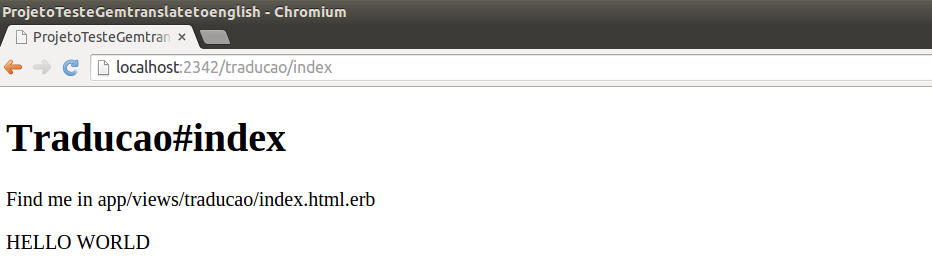
\includegraphics[scale=0.49]{images/resultado_de_translate_na_view.png}
  \caption{Resultado de Translate na View}
  \label{fig:resultado_de_translate_na_view}
\end{figure}
